\documentclass[border=5pt]{standalone}
\usepackage[T1]{fontenc}
\usepackage{lmodern,amsmath,amssymb,tikz}
\usetikzlibrary{arrows.meta,decorations.markings,calc,backgrounds}
\definecolor{branch}{RGB}{195,80,15}
\definecolor{branchB}{RGB}{18,125,105}
\definecolor{direct}{RGB}{37,82,156}
\definecolor{merged}{RGB}{109,57,133}
\definecolor{spoke}{RGB}{95,95,102}
\definecolor{srcgreen}{RGB}{22,120,55}
\tikzset{
  v/.style={circle,fill=black,inner sep=1.55pt},
  ins/.style={rectangle,draw=black,fill=white,line width=0.65pt,minimum size=4.6pt,inner sep=0pt},
  res/.style={line width=0.78pt,postaction={decorate},decoration={
    markings,
    mark=at position 0.48 with {\draw[line width=0.72pt,fill=white] (-0.27,-0.105) rectangle (0.27,0.105);},
    mark=at position 0.82 with {\arrow{Stealth[length=1.35mm,width=1.05mm]}}
  }},
  resns/.style={line width=0.78pt,postaction={decorate},decoration={
    markings,
    mark=at position 0.50 with {\draw[line width=0.72pt,fill=white] (-0.25,-0.10) rectangle (0.25,0.10);}
  }},
  source/.style={-{Stealth[length=1.55mm,width=1.15mm]},line width=0.75pt},
  reduce/.style={-{Stealth[length=2.0mm,width=1.45mm]},line width=0.9pt},
  lbl/.style={fill=white,inner sep=1.1pt}
}

\begin{document}
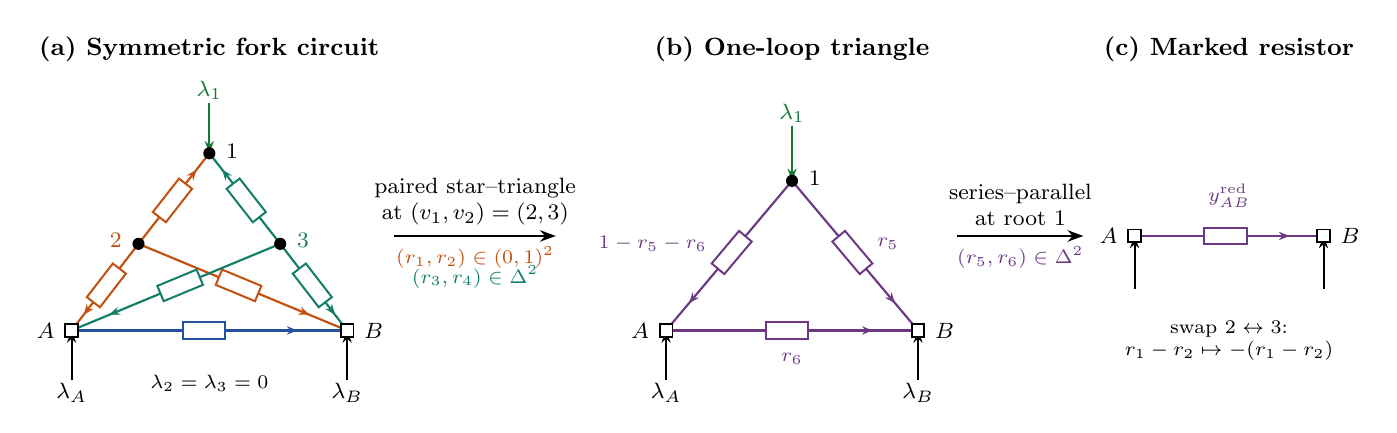
\begin{tikzpicture}[x=1cm,y=1cm,font=\footnotesize]

% Stage (a): Three-loop symmetric fork circuit
\begin{scope}[xshift=0cm]
  \node[font=\small\bfseries] at (1.85,3.92) {(a) Symmetric fork circuit};
  \coordinate (A) at (0.1,0.35);
  \coordinate (B) at (3.6,0.35);
  \coordinate (v1) at (1.85,2.60);
  \coordinate (v2) at (0.95,1.45);
  \coordinate (v3) at (2.75,1.45);

  \draw[res,direct] (A)--(B);
  \draw[res,branch] (v2)--(v1);
  \draw[res,branch] (v2)--(A);
  \draw[res,branch] (v2)--(B);
  \draw[res,branchB] (v3)--(v1);
  \draw[res,branchB] (v3)--(A);
  \draw[res,branchB] (v3)--(B);

  \draw[source,srcgreen] (1.85,3.24)--(v1);
  \node[srcgreen,above,inner sep=1pt] at (1.85,3.24) {$\lambda_1$};
  \draw[source] (0.1,-0.28)--(A); \node[below,inner sep=1pt] at (0.1,-0.28) {$\lambda_A$};
  \draw[source] (3.6,-0.28)--(B); \node[below,inner sep=1pt] at (3.6,-0.28) {$\lambda_B$};

  \node[right] at (1.94,2.63) {$1$};
  \node[branch,left] at (0.86,1.50) {$2$};
  \node[branchB,right] at (2.84,1.50) {$3$};
  \node[font=\scriptsize] at (1.85,-0.32) {$\lambda_2=\lambda_3=0$};

  \node[ins,label=left:$A$] at (A) {};
  \node[ins,label=right:$B$] at (B) {};
  \foreach \p in {v1,v2,v3}{\node[v] at (\p) {};}
\end{scope}

\draw[reduce] (4.20,1.55)--node[above,align=center]{paired star--triangle\\at $(v_1,v_2)=(2,3)$} node[below,align=center,font=\scriptsize]{{\color{branch}$(r_1,r_2)\in(0,1)^2$}\\[-1pt]{\color{branchB}$(r_3,r_4)\in\Delta^2$}} (6.25,1.55);

% Stage (b): Reduced one-loop triangle (1, A, B)
\begin{scope}[xshift=7.55cm]
  \node[font=\small\bfseries] at (1.70,3.92) {(b) One-loop triangle};
  \coordinate (A) at (0.1,0.35);
  \coordinate (B) at (3.3,0.35);
  \coordinate (v1) at (1.70,2.25);

  \draw[res,merged] (v1)--(A);
  \draw[res,merged] (v1)--(B);
  \draw[res,merged] (A)--(B);

  \draw[source,srcgreen] (1.70,2.95)--(v1);
  \node[srcgreen,above,inner sep=1pt] at (1.70,2.95) {$\lambda_1$};
  \draw[source] (0.1,-0.28)--(A); \node[below,inner sep=1pt] at (0.1,-0.28) {$\lambda_A$};
  \draw[source] (3.3,-0.28)--(B); \node[below,inner sep=1pt] at (3.3,-0.28) {$\lambda_B$};

  \node[right] at (1.79,2.28) {$1$};
  \node[merged,left,font=\scriptsize] at (0.74,1.45) {$1-r_5-r_6$};
  \node[merged,right,font=\scriptsize] at (2.66,1.45) {$r_5$};
  \node[merged,below,font=\scriptsize] at (1.70,0.18) {$r_6$};

  \node[ins,label=left:$A$] at (A) {};
  \node[ins,label=right:$B$] at (B) {};
  \node[v] at (v1) {};
\end{scope}

\draw[reduce] (11.35,1.55)--node[above,align=center]{series--parallel\\at root $1$} node[below,merged,align=center,font=\scriptsize]{$(r_5,r_6)\in\Delta^2$} (12.95,1.55);

% Stage (c): Marked resistor AB
\begin{scope}[xshift=13.50cm]
  \node[font=\small\bfseries] at (1.30,3.92) {(c) Marked resistor};
  \coordinate (A) at (0.1,1.55);
  \coordinate (B) at (2.5,1.55);
  \draw[res,merged] (A)--(B);
  \draw[source] (0.1,0.88)--(A);
  \draw[source] (2.5,0.88)--(B);
  \node[merged,above=2.4mm,font=\scriptsize] at (1.30,1.55) {$y_{AB}^{\mathrm{red}}$};
  \node[align=center,font=\scriptsize] at (1.30,0.22) {swap $2\leftrightarrow 3$:\\$r_1-r_2\mapsto -(r_1-r_2)$};
  \node[ins,label=left:$A$] at (A) {};
  \node[ins,label=right:$B$] at (B) {};
\end{scope}

\end{tikzpicture}
\end{document}
